%%%%%%%%%%%%%%%%%%%%%%%%%%%%%%%%%%%%%%%%%%%%%%%%%%%%%%%%%%%%%%%%%%%%%%
% How to use writeLaTeX: 
%
% You edit the source code here on the left, and the preview on the
% right shows you the result within a few seconds.
%
% Bookmark this page and share the URL with your co-authors. They can
% edit at the same time!
%
% You can upload figures, bibliographies, custom classes and
% styles using the files menu.
%
%%%%%%%%%%%%%%%%%%%%%%%%%%%%%%%%%%%%%%%%%%%%%%%%%%%%%%%%%%%%%%%%%%%%%%

\documentclass[12pt]{article}

\usepackage{sbc-template}

\usepackage{graphicx,url}

%\usepackage[brazil]{babel}   
\usepackage[utf8]{inputenc}  

     
\sloppy

\title{Instructions for Authors of SBC Conferences\\ Papers and Abstracts}

\author{Luciana P. Nedel\inst{1}, Rafael H. Bordini\inst{2}, Flávio Rech
  Wagner\inst{1}, Jomi F. Hübner\inst{3} }


\address{Instituto de Informática -- Universidade Federal do Rio Grande do Sul
  (UFRGS)\\
  Caixa Postal 15.064 -- 91.501-970 -- Porto Alegre -- RS -- Brazil
\nextinstitute
  Department of Computer Science -- University of Durham\\
  Durham, U.K.
\nextinstitute
  Departamento de Sistemas e Computação\\
  Universidade Regional de Blumenal (FURB) -- Blumenau, SC -- Brazil
  \email{\{nedel,flavio\}@inf.ufrgs.br, R.Bordini@durham.ac.uk,
  jomi@inf.furb.br}
}

\begin{document} 

\maketitle

\begin{abstract}
  This meta-paper describes the style to be used in articles and short papers
  for SBC conferences. For papers in English, you should add just an abstract
  while for the papers in Portuguese, we also ask for an abstract in
  Portuguese (``resumo''). In both cases, abstracts should not have more than
  10 lines and must be in the first page of the paper.
\end{abstract}
     
\begin{resumo} 
  Este meta-artigo descreve o estilo a ser usado na confecção de artigos e
  resumos de artigos para publicação nos anais das conferências organizadas
  pela SBC. É solicitada a escrita de resumo e abstract apenas para os artigos
  escritos em português. Artigos em inglês deverão apresentar apenas abstract.
  Nos dois casos, o autor deve tomar cuidado para que o resumo (e o abstract)
  não ultrapassem 10 linhas cada, sendo que ambos devem estar na primeira
  página do artigos.
\end{resumo}

\section{Introdução}\label{sec1}

\section{Outro Capitulo} \label{sec2}

\section{Metodologia: Planejamento da Revisão Sistemática} \label{sec3}

Segundo Kitchenham \cite{kitchenham2004procedures} a maior parte das pesquisas começa com uma revisão de literatura, no entanto, para ter valor científico é necessário que essa revisão seja feita de forma abrangente, não tendenciosa, aberta e objetiva. Por isso a necessidade de utilizar a revisão sistemática, que deve identificar, interpretar e avaliar todas as pesquisas disponíveis e relevantes sobre uma questão \cite{keele2007guidelines}. Para isso a revisão sistemática segue um protocolo de busca, que deve conter todas as informações que permitam que a revisão seja repetida por outros pesquisadores interessados no trabalho desenvolvido.

De acordo com \cite{brereton2007lessons} a revisão sistemática envolve três fases, resumidamente as fases são: Planejamento, Execução e análise dos resultados. Neste trabalho cada faze aborda:

 \begin{itemize}
   \item  \textbf{Planejamento: } Identificação  das  necessidades  para  a  revisão  e  elaboração do protocolo, o protocolo que deverá orientar toda a revisão sistemática. Nele deve conter as informações sobre o objetivo, a descrição do problema, as questões
da pesquisa e os métodos e critérios utilizados para a busca, seleção, avaliação e extração de dados.
   \item  \textbf{Execução: } Na fase de execução, os métodos descritos no protocolo são aplicados e documentados, além da identificação da pesquisa, seleção e avaliação da qualidade  dos  estudos.
      \item  \textbf{Análise dos Resultados: }Na fase de análise dos resultados os dados dos estudos são extraídos e sintetizados e os
resultados são analisados.
 \end{itemize}

\subsection{Objetivos} \label{sec3:subsec1}

O objetivo deste trabalho....

\subsection{Questão de Pesquisa} \label{sec3:subsec2}

A partir do objetivo estabelecido na Seção \ref{sec3:subsec1}, foram elaboradas as seguintes questões de pesquisa:

 \begin{itemize}
   \item  \textbf{H1: }
   \item  \textbf{H2: }
 \end{itemize}

Essas questões deverão ser respondidas ao final da revisão sistemática.

\subsection{Métodos de Busca de Publicações} \label{sec3:subsec3}

Esta  Subseção  descreve  onde  e  como  foram  realizadas
as  buscas  desta  pesquisa. Apresentam-se também as palavras-chave utilizadas para a geração da string  de busca e os idiomas aceitos para a seleção dos resultados. 

As fontes selecionadas para realização deste trabalho foram pesquisadas nas bases eletrônicas de dados disponíveis no portal CAPES, incluindo documentos indexados nas seguintes bases:

 \begin{itemize}
   \item  \textbf{ACM digital library}
   \item  \textbf{IEEEXplore}
   \item  \textbf{Springer}
   \item  \textbf{Google Scholar}
 \end{itemize}
 
As seguintes palavras foram utilizadas para fazer as buscas de estudos:

 \begin{itemize}
   \item  \textbf{Agile}
   \item  \textbf{Deploy}
   \item  \textbf{Process Software Deployment}
   \item  \textbf{Devops}
   \item  \textbf{Continuous Delivery}
 \end{itemize}

Com o intuito de abordar as palavras chave anteriormente definidas, foram definidas as seguitnes strings de busca:

 \begin{itemize}
   \item  \textbf{("deploy" or "deployment") AND  "agile" AND "process software" }
    \item  \textbf{("deploy" or "deployment") AND  "agile" AND "continuous delivery"}
    \item  \textbf{ "process" AND  "agile" AND  "deployment" AND "software"}
 \end{itemize}

É importante ressaltar que as strings de busca deverá na medida do possível ser igual em todas as máquinas de busca, contudo poderá existir adaptações mas levando em consideração que a string adaptada deverá ser logicamente equivalente a string original.

O idioma escolhido foi o Inglês, também considerou-se qualquer tipo de trabalho ou artigo que fizesse abordagem sobre características de implantação de software no contexto de métodos ágeis.
   

\subsection{Critérios de Seleção} \label{sec3:subsec4}

Após a realização das buscas, serão incluídos na revisão todos os artigos encontrados com a utilização do método descrito na subseção \ref{sec3:subsec5} que satisfaçam todos os seguintes critérios de inclusão:

 \begin{itemize}
   \item  \textbf{Critério de inclusão:} O resultado deve estar no indoma inglês.
   \item  \textbf{Critério de inclusão:}  O resultado deve estar disponível integralmente.    
   \item  \textbf{Critério de inclusão:}   O resultado deve conter no título, ou resumo, ou conclusão,  informações relevantes sobre o tema desse trabalho.
 \end{itemize}
 
 Após a realização das buscas, serão excluídos na revisão todos os artigos que satisfaçam todos os seguintes critérios de inclusão:

 \begin{itemize}
   \item  \textbf{Critério de exclusão:} O resultado não trata do contexto de implantação e desenvolvimento de software.
 \end{itemize}
 
\subsection{Procedimentos Para Extração de Dados} \label{sec3:subsec5}

Foi realizado uma busca em inglês em cada uma das fontes definidas na seção \ref{sec3:subsec3}, utilizando as strings de busca definidas na seção \ref{sec3:subsec3}, a partir da busca foram lidos todos os títulos, ou resumos, ou conclusões dos artigos encontrados. Isso foi necessário para saber quantos passaram pelos critérios de inclusão e quais não foram de acordo com os critérios de exclusão, citados na seção \ref{sec3:subsec4}, ou seja, aqueles trabalhos que os resultado não continham relevância no título, ou resumo, ou conclusão foram exluídos.

\subsection{Extração de Resultados} \label{sec3:subsec6}

Após  esta leitura inicial ,  os  resultados que foram incluídos a partir dos critérios de inclusão foram  selecionados  para  serem  lidos e  analisados de forma integral, assim os resultados aprovados pelos critéios de inclusão serão considerados neste estudo.

\section{Execução da Revisão Sistemática} \label{sec4}

\subsection{Execução das Buscas} \label{sec4:subsec1}

\subsection{Seleção Preliminar} \label{sec4:subsec2}

\subsection{Seleção Final} \label{sec4:subsec3}

\section{Análise dos resultados} \label{sec5}

\section{Conclusão} \label{sec6}

\section{Figures and Captions}\label{sec:figs}

\begin{table}[ht]
\centering
\caption{Variables to be considered on the evaluation of interaction
  techniques}
\label{tab:exTable1}
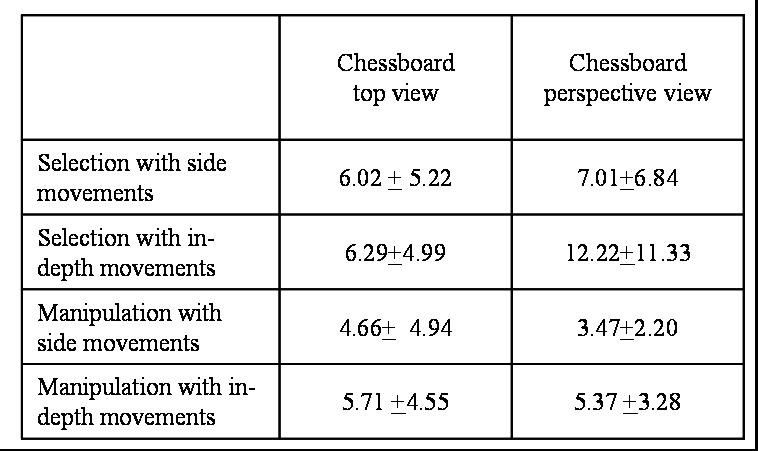
\includegraphics[width=.7\textwidth]{table.jpg}
\end{table}

\section{References}
\bibliographystyle{sbc}
\bibliography{sbc-template}

\end{document}
